\documentclass[a4paper,10pt]{article}

\usepackage{graphicx}
\usepackage[ansinew]{inputenc}
\usepackage[spanish]{babel}
\usepackage{fancyhdr} % Para tener cabecera y pie de página con un estilo personalizado:
\usepackage{pdfpages} % Para importar PDF 

\title{		\textbf{Trabajo Práctico - Etapa 1 \\ \textit{Voto Electrónico}} }

\author{	Martín Hernán Gómez, \textit{Padrón Nro. 85.780}                     \\
            \texttt{martinhgomez@yahoo.com.ar}                                              \\[2.5ex]
            Ignacio Marambio Catán, \textit{Padrón Nro. 82.694}                     \\
            \texttt{ignacio.marambio@gmail.com}                                             \\[2.5ex]
            aaa, \textit{Padrón Nro. 00000}                     \\
            \texttt{a@a.com }                                              \\[2.5ex]
            Daniel Shlufman, \textit{Padrón Nro. 88.040}                     \\
            \texttt{incorporado@gmail.com}                                              \\[2.5ex]
            Lucas Damian Tarcetti, \textit{Padrón Nro. 87.165}                     \\
            \texttt{lucas.tarcetti@yahoo.com.ar}                                              \\[2.5ex]
            \normalsize{2do. Cuatrimestre de 2011}                                      \\
            \normalsize{75.06 Organización de Datos $-$ Cátedra Lic. Arturo Servetto}  \\
            \normalsize{Facultad de Ingeniería, Universidad de Buenos Aires}            \\
       }
\date{26/10/11}



\begin{document}

\maketitle
\thispagestyle{empty}   % quita el número en la primer página
\newpage

\tableofcontents
\newpage


\pagestyle{fancy} % A partir de acá Encabezados y pes de pagina con formato
\section{Introducción}

El trabajo consiste crear una aplicación capaz de mantener un sistema de voto electrónico.

\subsection{Objetivos}

El objetivo de este trabajo práctico es que la aplicación sea capaz de mantener información sobre las entidades que componen el sistema de votaciones (votantes, elecciones, candidatos, etc.), y de proveer la posibilidad a un votante de emitir su voto para la correspondiente elección.


\section{Documentación técnica}


\subsection{Elección del lenguaje de programación}
La resolución del trabajo práctico debe será realizada en plataforma Linux y en lenguaje C++, aprovechando el uso de la programación orientada a objetos.

\subsection{Entidades}

\begin{itemize}
\item Distrito ((distrito)i)
\item Votante ((DNI)i, NombreyApellido, clave, domicilio, (distrito)ie, ((eleccion)ie)*)
\item Eleccion ((fecha, (cargo)ie)i, ((distrito)ie)+)
\item Lista (((eleccion)ie, nombre)i, cantidadVotos)
\item Candidato (((lista)ie, (votante)ie, (cargo)ie)i)
\item Cargo ((cargo)i)
\item Administrador ((usuario)i, clave)
\end{itemize}

\subsection{Estructuras de datos}
	Las estructuras principales elegidas para este trabajo han sido elegidas según la necesidad de cada entidad. Las mismas son:

\begin{itemize}
\item Árbol B+
\item Dispersión Extensible
\item Archivos de Bloques
\item Registros Variables
\end{itemize}	
	
\subsection{Funcionalidades}
En el ámbito del administrador se encuentran las siguientes funcionalidades:

\begin{itemize}
\item Mantener Distritos
\item Mantener Votantes
\item Mantener Elecciones
\item Mantener Cargos
\item Mantener Listas
\item Mantener Candidatos
\item Informar Resultados
\end{itemize}	

\subsection{Descripción de la arquitectura utilizada}

Para una mejor observación de los diagramas de clases de la arquitectura utilizada en el programa, las mismas se encuentran documentadas en un archivo externo junto con su descripción, se puede acceder a el a través del archivo `00 Index.html', el mismo se encuentra en la carpeta `Documentación'. Desde allí se puede navegar a través de todas las clases existentes.


\subsection{Descripción de cada clase utilizada}

    A continuación se enumeran las principales clases de la aplicación, no refiréndonos a sus nombres de archivo sino con su nombre conceptual.

\begin{itemize}
\item Clase ArbolBMas: Se utiliza para guardar las listas de votación y para la confección de informes.
\item Clase Dispersión: Se utiliza para almacenar todas las demás entidades que no sean las listas de votación.
\item Clase Archivo en Bloques: Se usa para darle un sustento en disco a las clases de Árbol B+ y de Dispesión. Ofrece una persistencia en disco en un archivo de bloques.
\item Clases de Entidades: Las mismas se utilizan para instanciar cada entidad necesaria al momento de crear una votación. Las mismas incluyen: Distrito, Votante, Eleccion, Lista, Candidato, Cargo, Administrador.
\end{itemize}	


\subsection{Justificación de uso de cada clase utilizada}
    El uso del \textit{Árbol B+} se eligió principalmente debido a la opción de poder hacer búsquedas parciales y además a la ventaja de poder acceder secuencialmente a los datos de forma ordenada.
    El uso del \textit{archivo de dispersión} se eligió debido a que usa la menor cantidad de accesos posibles (solo un acceso) haciendo que se optimice el uso de estos archivos, al ser los mas accedidos en disco.
    El uso del \textit{archivo de bloques} se eligió por ser el más compatible con respecto a la persistencia del Árbol B+ y del archivo de dispersión, haciendo mas efectivo el uso de los mismos.

\subsection{Archivos auxiliares}
Definiciones lógicas y físicas de todos los archivos que se utilicen (datos maestros, índices, trabajo, control, etc).Descripción de la organización de cada uno de los archivos.  Para qué se utiliza. Por qué se utiliza (base teórica).

Dentro de los archivos utilizados para el funcionamiento del programa disponemos de las siguientes estructuras auxiliares:

\begin{itemize}
\item Archivo de configuración: El mismo se usa para obtener las rutas de los archivos de dispersión, archivo del árbol, tamaños de cubetas y de nodos.
\item Índice: El índice se usa para la obtención de los informes de votaciones por distintos criterios de una misma base de datos.
\item Archivo de control: Se utiliza para poder persistir datos referentes a las estructuras de control de las estructuras, como por ejemplo la tabla de dispersión dentro de la estructuras de dispersión.
\item Archivo de password: Guarda el \textit{user} y \textit{pass} perteneciente al administrador de votos.
\end{itemize}	

\subsection{Planificación de tareas}
Planificación (identificación de tareas, estimación de duración y asignación)

A grandes rasgos la planificación del proyecto se realizó dentro de las cinco semanas la siguiente manera:

\begin{itemize}
\item Semana 1: Planeamiento del problema, elección de las distintas estructuras para las entidades existentes, configuración del sistema operativo, herramientas de compilación, IDE's, etc. Para su correcto funcionamiento en el sistema Linux. Duración aproximada: 1 semana.
\item Semana 2: Construcción de las entidades, creación de sus respectivas clases (1 semana). Creación de la clase encargada del manejo en disco, manejador de archivos (1 semana). Comienzo de creación de la clase de Árbol B+ (4 semanas).
\item Semana 3: Comienzo de creación de la clase de Dispersión (3 semanas). Creación de la clase encargada del archivo de bloques (2 semanas). Creación de clase bucket y creación de clase nodo.
\item Semana 4: Creación de pruebas individuales e integrales (1 semana). Serialización e hidratación de datos (1 semana). Creación del archivo de buckets (1 semana).
\item Semana 5: Integración de los distintos módulos (1 semana). Creación de la lógica de votación (1 semana). Implementación de una interfaz para el usuario (1 semana).
\end{itemize}


\subsection{Bugs conocidos}

A continuación se enumeran ciertas situaciones donde el programa podría presentar dificultades en su proceso:

\begin{itemize}
\item La fechas deben tener tener el formato: aaaa/mm/dd para poder procesarse correctamente.
\item Si el archivo de configuración no tiene el delimitador `//' dentro del archivo, el mismo no parsea ningún dato, ya que toma al archivo entero como comentario
\item El archivo de bloques debido a su estructura interna debe tener un tamaño de bloque que sea múltiplo de 4 bytes, si no es de esta forma podría referenciar erroneamente a un bloque. Esto se solucionó validando el tamaño de bloque al iniciar un archivo.
\item En una elección determianda se podría agregar cualquier distrito sin que se verifique si realmente existe.
\item El borrado de algún archivo de control, configuración y/o datos en tiempo de ejecución llevará a una malfunción del programa.
\end{itemize}


\subsection{Archivos de Control para las Entidades}

\subsubsection{Archivos de Control}

Se encuentran todos dentro de un directorio, especificado a través de un archivo de configuración de la aplicación, y pueden tener jerarquía de subdirectorios interna. Es donde se guarda toda la información necesaria para poder funcionar.

\subsubsection{Archivos con resultados}

Como respuesta a toda interacción, el sistema generará archivos de registro de operaciones (LOGs) en el directorio donde se llame a la aplicación.

\section{Parte teórica}

En la siguiente sección se enumeran distintos conceptos teóricos acerca de las estructuras usadas en la resolución del TP.

\subsection{Física - Organización}

\subsubsection{Organización de registros}
\begin{itemize}
\item La longitud de un registro y/o de un campo variable se delimita con el uso de un indicador de longitud, el cual se antepone a los datos pertenecientes al registro o campo. De esta forma se puede conocer donde termina la sección de datos.
\item En todos los casos se guarda como mínimo la información correspondiente a la longitud del segmento de datos pudiendo, en ciertos casos, guardarse mas información, según sea la estructura.
\end{itemize}


\subsubsection{Consideraciones acerca del Archivo de Bloques}

\begin{enumerate}
\item Los bloques tienen tamaño fijo, determinado por primera y única vez al crearse el archivo.
\item Existen 4 tipos de bloques: Data, Metadata, Removed y Head
\item Head: Existe un solo bloque de este tipo por archivo y siempre se ubica al principo del mismo (en la posición 0).

El bloque Head tiene en su estructura: 

$\vert$currmetadata (int)$\vert$maxblocknum(int)$\vert$blocksize(int)$\vert$ Espacio sin uso (int)$\vert$...
...$\vert$Espacio sin uso (int)$\vert$  
\item Data: Este bloque se usa íntegramente para guardar datos del usuario

El bloque Data tiene en su estructura: 

$\vert$datos(int)$\vert$...$\vert$datos(int)$\vert$...$\vert$datos(int)$\vert$
(Todo el espacio reservado para datos, sin metadata).
\item Metadata: Bloque que se encarga del control de los bloques de datos borrados (Removed). Aquí se guardan las referencias a bloques removed.

El bloque de Metadata tiene en su estructura: 

$\vert$ Metadata Anterior(int)$\vert$ currPos(int)$\vert$ ID bloqLibre (int)$\vert$ ...$\vert$ ID bloqLibre (int)$\vert$ 
\item Removed: Son bloques de datos que han sido borrados por el usuario, no se utiliza ningún atributo para identificarlos, los mismos están referenciados en el bloque de metadata como 'libre'.
\item Internamente todos los atributos de metadata son manejados como int. En el caso donde desde afuera se piden los bloques de datos el bloque se obtiene como un char*.
\item El currpos empieza desde el primer byte del bloque, incluyendo los bytes cabezeras. O sea que el 1er dato de metadata está en el byte 8 (2*sizeof(int))
\item Cada vez que cambia el 'currmetadata' o 'maxblocknum' se escribe en disco con serializehead (que escribe 2 veces en disco por cada vez que se lo llama)
\item Cada vez que cambia el 'currpos' se escribe en disco (se escribe en el bloque de metadata). Esto sucede al pedir un bloque nuevo o al borrar un bloque de datos
\item Está contemplado el caso donde el metadata actual no tiene bloques libres, y entonces este mismo pasa a ser un bloque disponible (Caso límite).
\item Está contemplado el caso donde borro un data, pero el metadata actual está totalmente lleno, pasando el bloque 'D' a ser un bloque 'M' (Caso límite).
\item Si pido un metadata nuevo tengo que ver si es el 1ro, si esto es así, su valor "anterior" (posición [1] dentro del bloque de int's) tiene que ser = Cero
\item No hace falta un getblock de 'R' porque esos bloques siempre van a ser accedidos a través de newblock (con parámetro 'D' o 'M')
\item No hace falta un newblock de 'R' porque esos bloques siempre van a ser creados a través de delblock
\item En una primera instancia, se propuso etiquetar cada bloque para su identificación. Pero luego, para simplificar el funcionamiento y para no invadir espacio en el bloque de Datos, se optó por no usar etiquetas en los bloques.
\end{enumerate}


\subsection{Índices - Búsqueda}

\subsubsection{Hashing}
Función de hashing utilizada. Criterio de elección. 

Para una rápida recuperación de la información se decide organizar dicho archivo con el método de dispersión extensible. Se utiliza un hashing extensible de valores sufijos. La función de hashing utilizada es f(x) = (x) mod (tamaño de tabla) 


\subsubsection{Árbol B+}
Nuestro arbol B+ es relativamente genérico, a excepción de la clave de ordenamiento que es invariablemente un string, los datos son una entidad genérica y en general no me interesa que se guarda ahi.

Está implementado de tal manera que también esta separado casi completamente de la parte que lidia con el almacenamiento teniendo 2 precondiciones ineludibles. el lugar donde se encuentra alojada la raíz debe ser invariante y las estructuras que representan a los punteros a los bloques deben ser representadas como enteros.

La separación se logró mediante la clase ffile y tuvo tanto éxito que con mínimas modificaciones fue posible pasar de un árbol cuyo almacenamiento era la memoria a otro cuyo almacenamiento era un archivo de bloques.

El árbol esta implementado en 4 clases diferentes, la ya mencionada ffile, bplustree, inner  $\_$node y leaf$\_$node estando estas ultimas intimamente relacionadas de manera tal que una esta declarada como friend de la otra. Esta decision se tomo para no exponer cosas criticas de las clases que necesariamente tenian que usarse entre inner$\_$node y leaf$\_$node.

En memoria, estas clases utilizan un vector de pares de enteros y cadenas de caracteres para los nodos internos (la clase inner$\_$node) y pares de cadenas y vectores en las hojas (la clase leaf$\_$node). Estas 2 clases, al serializarse se transforman en una cadena larga de caracteres (que se guarda en un vector) representada por pares longitud, datos. Ademas a esto se agrega un entero mas que representa la cantidad de pares, longitud, datos que existen en la cadena en adicion a un encabezado que es una I o una L segun sea el nodo un nodo interno o una hoja y un par de enteros mas que representan el nodo que contiene los datos cuya clave es mayor al nodo actual o el nodo que tiene datos menor al primer par del nodo.

En este momento, el árbol se comporta como un árbol B+ clásico para los agregados pero no hace rebalanceos en caso de los borrados.

Mas alla de los enteros que tienen tamaño fijo, el resto de las estructuras son dinamicas. El objetivo de esta implementacion fue utilizar la mayor cantidad de las funciones de la STL que fueran posible y, como desafortunadamente, la STL, si bien tiene una funcion de busqueda que funciona en contenedores como los vectores utilizados para almacenar los datos en la memoria de este árbol, ésta solo devuelve si un dato se encuentra o no en el contenedor pero no su posición o sus datos por lo que la búsqueda dentro de los nodos es lineal.

Esto también fue una pre condicion para poder implementar la función que luego de una búsqueda devuelva el dato inmediatamente mayor al ultimo devuelto.

Para ordenar los datos en memoria, sin embargo si se utiliza la función sort() del grupo de funciones incluidas en $<$algorithms$>$

\section{Documentación de usuario}

\subsection{Instalación del sistema}

La instalación usará un archivo makefile, el cual realizará automaticamente toda la operación de compilación de todos los archivos de código fuente, recorriendo todas las subcarpetas necesarias para una operación exitosa.

Para la instalación del sistema debemos descomprimir el archivo conteniendo el código fuente en la carpeta donde se desea realizar la misma. Una vez realizada la descompresión debemos ejecutar por consola, situados en la ruta elegida, el comando \textit{make} el cual compilará todos los archivos fuente y como consecuencia obtendremos el archivo ejecutable listo para usar.

\subsection{Ejecución del sistema}

    Una vez creado el archivo ejecutable debemos iniciar el programa\footnote{Para iniciar el programa, al administrador se debe autentificar. User: undomiel, Pass: aragorn} pasando por parámetro la ruta del archivo de configuración, esto es un requisito obligatorio para comenzar con el programa, mediante los argumentos -c  $<$rutaArchivoConfiguración$>$. De esta forma, desde el directorio donde se creó el ejecutable, se inicia el sistema:

\begin{quote}
 ./voto -c ../ArchivosAuxiliares/config.txt
\end{quote}
\textbf{Nota:} -c es el flag para ubicar el archivo de configuración. Para ver las demás opciones podemos ingreasar al programa con -h

A su vez el archivo de configuración proveerá todos los requisitos necesarios para ubicar los demás archivos relativos al programa, ya sean archivos de datos, control, configuración o el archivo de password.


\subsubsection{Interfaz de administrador}

Al iniciar el programa el administrador de la votación deberá autenticarse para poder entrar al sistema, una vez ingresado tendrá un menú con opciones donde podrá:

\begin{itemize}
\item Mantener Distritos.
\item Mantener Votantes.
\item Mantener Elecciones.
\item Mantener Cargos.
\item Mantener Listas.
\item Mantener Candidatos.
\item Informar Resultados.
\end{itemize}


\subsubsection{Interfaz de usuario}

Una vez iniciada una votación, se dispondrá de una interfaz para el usuario 'votante'. En esta instancia el votante podrá:

\begin{itemize}
\item Autenticarse
\item Emitir voto
\item Corregir voto
\item Informar voto
\end{itemize}

\newpage


\section{Segunda etapa - Seguridad}

\subsection{Método de Vigènere}

\subsubsection{Resolución del método}

Se empleará el método para cifrar los reportes generados: Listas, Elección, Distrito.

Para la resolución se necesitará generar una clave k de dimensión n. Cada elemento de la clave pertenece al alfabeto sobre el cual se resuelve el método.

Una opción resulta en considerar al alfabeto como todo el conjunto de los elementos representables con 1 byte, es decir 256 elementos. De esta forma se trabaja con aritmética modular de modulo 256.

Desde el punto de vista de la programación se crearía la clase Vigènere que sería la encargada de realizar la encriptación ( y desencriptación ) de un documento.

El criptosistema es simétrico por lo que al instanciar la clase se le asignaría la clave que podría ser del tipo vector. Se define implícitamente el tamaño del alfabeto que resulta ser de 256, correspondiente al código ASCII.

La clave se pasa por valor de forma tal que el objeto instanciado tenga un copia interna de la clave y pueda manejarse sin riesgo de que en el caso de ser pasado por referencia se elimine accidentalmente.

La encriptación manejaría strings, recibiría en mensaje y lo cifraría devolviendo el correspondiente criptograma. De esta forma haríamos que se desentienda del origen del objeto que está manejando, que podría ser desde memoria o desde disco.

El descrifrador recibe el criptograma, lo descifra con la clave y devuelve el mensaje como un string.

Hay dos situaciones diferentes en las cuales se debe usar Vigeneré. Una es para cifrar un texto plano. La otra es para cifrar un texto plano y a continuación otro texto plano utilizando la misma instancia de Vigeneré y la misma clave.

En el caso que se quiere cifrar un texto plano solamente con la misma clave y la misma instancia de Vigeneré: para el manejo en bloques Vigenere cuenta con dos variables que contienen la última posición de la clave durante el uso del cifrador y del descifrador, de forma tal que no haya que restringir el mensaje que se desea encriptrar/descencriptar a un tamaño múltiplo del tamaño de la clave porque cada vez que se llega a la última posición del cifrador/descifrador se reinicia esta variable.

\subsubsection{Criptoanálisis}


Para realizar el criptoanálisis una opción es resolverlo empleando el método de Kasiski.

1. Desarrollo del método:

El método consiste en realizar una búsqueda de fragmentos de bits repetidos para luego calcular la distancia que los separa. A partir de ello se obtiene el máximo común divisor MCD para obtener la dimensión de la clave.

Una vez obtenida se procede a realizar un análisis de frecuencia de caracteres en una forma especial. Se tienen tantos vectores (o listas) como lo indique la dimensión de la clave. Se aplica la operación de módulo sobre la posición del elemento en el flujo de caracteres, y se asigna la frecuencia correspondiente al elemento encontrado en el vector correspondiente, que se identifica por el resultado de la operación módulo.

Luego conociendo previamente el idioma en que se encuentra el criptograma, se procede a buscar los caracteres con mayores frecuencias.

Como tenemos 256 posibilidades, hacemos un prueba sobre un archivo para obtener un histograma de las frecuencias de las apariciones de los códigos ASCII en un texto.

En base a pruebas realizadas por el grupo se obtuvo el siguiente gráfico:
\begin{center}
\begin{figure}[h] %[h] para here [b] para bottom [t] para top
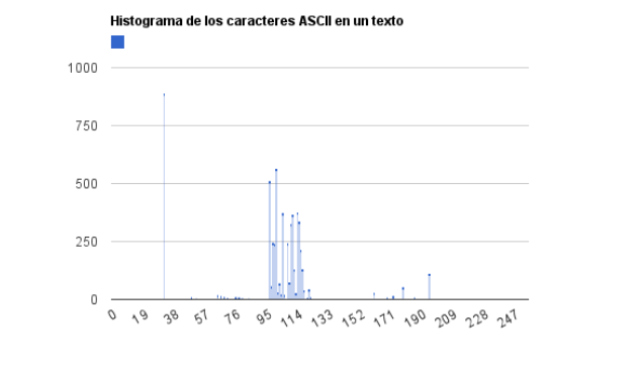
\includegraphics[scale=0.5]{./histo.jpg}
\end{figure}
\end{center}

El gráfico que se observa muestra las frecuencias obtenidas en una prueba para los 255 caracteres ASCII. En el gráfico no se puede observar claramente pero se observa que se encuentran entre el 42 y el 126 que corresponde a los caracteres imprimibles. Por otro lado, hay un pico muy elevado que corresponde al caracter 32 que resulta ser el espacio.

Luego se analiza el mismo gráfico pero acotado a los valores imprimibles. En este caso, el caracter con mayor frecuencia es el 32, que resulta ser el espacio, seguido del caracter e (101), el caracter a(97) y por último el caracter o(111). Estos son los más frecuentes y dependiendo del archivo la frecuencia puede variar levemente.

En el texto de prueba se obtuvieron en porcentaje:
\begin{itemize}
\item espacio:16\%
\item a: 9\%
\item e: 10\%
\item o: 6,7\%
\end{itemize}

Es decir que como es esperable las minúsculas son más probables que las mayúsculas, y el caracter espacio es el más probable. Esta información es de suma utilidad al realizar el análisis de frecuencias que requiere el método.

Es destacable que con sólo los caracteres espacio, a, e y o se emplean en el 36\% de un texto.

Finalmente se descifra el mensaje.

\subsection{Método RSA}

\subsubsection{Resolución del método}

Se empleará el método para cifrar los datos de los votantes.

El sistema empieza generando por primera y única vez el par de claves privada y pública que son guardadas en un archivo en disco.

\paragraph{Utilizacion de campos finitos en el algoritmo de RSA}

Se utilizará el algoritmo de euclides extendido para generar el inverso multiplicativo o sea el número que se utilizará para desencriptar y que por lo tanto compondrá la clave privada.

También se usará exponenciación por cuadrados para la operación $a^b$ mod q .

Por esta razón se debe tener especial cuidado en la cantidad de bits que se utilizará para representar los números ya que si se trabaja con números demasiado grandes las operaciones de campos finitos pueden fallar. Por esto el enunciado al pedir que se ingrese el tamaño del número da la posibilidad de limitar este tamaño.

Limitaremos el tamaño de los números primos a entre 3 y 97. Siendo los demás números resultados de operaciones de campos finitos de tamaño manejable por el algoritmo de RSA.

\paragraph{Objeto RSA}

Desde el punto de vista de la programación se crearía la clase RSA que será la encargada de realizar la encriptación/desencriptación de los datos del votante.

\paragraph{Encriptación}
El votante instancia un objeto RSA con sus atributos cargados apartir de un archivo.

La encriptación se realiza sobre el string serializado del votante.

Desde serializar se llama al método de encriptación de RSA pasándole el string serializado.

Se toma cada caracter del string y se lo convierte en número entero.

Se realizan las operaciones de campos finitos y se devuelve un numero grande.

Se almacena el número grande en un buffer auxiliar.

Luego de almacenar todos los caracteres transformados en numeros en el buffer auxiliar, se devuelve el string asociado a este buffer de numeros grandes.

Todos los votantes se cifran con la misma clave, ésta se genera una única vez y se almacena en un archivo aparte. Cada vez que se desee encriptar se buscará la clave pública en el archivo. De esta forma al desencriptar se evita tener que realizar una búsqueda de la clave que cifró cada votante ya que es la misma para todos.

\paragraph{Desencriptación}
El deserializar de votante recibe el string serializado y encriptado.

El deserializar de votante instancia un objeto RSA.

Se inicializan los atributos del RSA apartir de la clave privada y pública guardadas en un archivo.

Se desencripta el string que recibió el deserializar de votante a partir del método desencriptar de RSA.

Desencriptar recibe el string serializado y encriptado y procede a desencriptar cada caracter del string casteado a un numero grande.

Se realizan las operaciones de campos finitos y se devuelve un numero entero.

Cada número entero (caracter desencriptado) se carga en un string. Al final se devuelve este string desencriptado que es el que el deserializar procede a hidratar.



\subsubsection{Criptoanálisis}
Se genera una lista de números primos entre 3 y 97 dado que hemos decidido acotar los números primos a este rango.

Se realizan multiplicaciones entre todos los numeros hasta lograr encontrar el par que de como resultado el n de las claves.

El ataque por fuerza bruta es el más sencillo y eficaz dado el pequeño rango de números posibles. Por eso se recomienda que los números primos sean de 1024 bits al menos así dificulta la capacidad de la computadora de realizar operaciones matemáticas en un tiempo razonable o útil.

\newpage


\section{Corridas de prueba - 1er Etapa}

A continuación se detallan las pruebas realizadas sobre el funcionamiento del programa. Se emplearon las pruebas detalladas en el enunciado del informe, las cuales pasaron con éxito.

\paragraph{Corridas de prueba}

\begin{verbatim}

Ingreso:
INGRESO APROBADO
Bienvenido al sistama de gestion de elecciones
¿ Desea eliminar la base de datos y comenzar de 0? S/N
S

Menú principal:
Opciones: 

1) Mantener Distritos
2) Mantener Votantes
3) Mantener Elecciones
4) Mantener Cargos
5) Mantener Listas
6) Mantener Candidatos
7) Informar Resultados
8) Habilitar Elecciones
9) Habilitar Votantes para elección
10) salir
Opcion: 1

Menú de Distrito:
Opciones: 

1) Alta Distrito
2) Baja Distrito
3) Modificar Distrito
4) Volver atrás
5) Ver Distritos
Opcion: 1

Ingrese el nombre del distrito: 
Misiones

Operacion OK

Menú de Votante:
Opciones: 

1) Alta Votante
2) Baja Votante
3) Modificar Votante
4) Volver atrás
5) Alta Automática
6) Ver votantes
Opcion: 1

Ingrese el DNI del votante: 14254983

Ingrese nombre: Daniel

Ingrese apellido: Martinez

Ingrese la clave: 8754

Clave: 8754
Ingrese el domicilio: San Luis 2728

dom: San Luis 2728
Ingrese el nombre del distrito: 
Misiones

Distrito: Misiones
Operacion OK

Opciones: 

1) Alta Votante
2) Baja Votante
3) Modificar Votante
4) Volver atrás
5) Alta Automática
6) Ver votantes
Opcion: 5

Ingrese la cantidad de votantes a ingresar: 3
 - Nombre: Mariel Iacub
 - DNI: 1
 - Password: 8335
 - Domicilio: Haiti 2793
 - Distrito: Jujuy
Elecciones Anteriores: 
---------------------- 
El votante no participo de ninguna eleccion a la fecha

 - Nombre: Ivan Lopez
 - DNI: 2
 - Password: 6498
 - Domicilio: Montiel 3061
 - Distrito: Santa Fe
Elecciones Anteriores: 
---------------------- 
El votante no participo de ninguna eleccion a la fecha

 - Nombre: Fernanda Rodriguez
 - DNI: 3
 - Password: 4940
 - Domicilio: Udaondo 1425
 - Distrito: Ciudad Autonoma de Buenos Aires
Elecciones Anteriores: 
---------------------- 
El votante no participo de ninguna eleccion a la fecha

Menu de Cargo:
Opciones: 

1) Alta Cargo
2) Baja Cargo
3) Modificar Cargo
4) Volver atrás
5) Ver cargos
Opcion: 1

Ingrese el nombre del cargo principal: 
Presidente

Desea agregar subcargos? (S/N)S

Ingrese el nombre del subcargo: 
Vice Presidente

Desea agregar más subcargos? (ingrese 'S' para seguir)N

Operacion OK

Menú de Elección:
Opciones: 

1) Alta Eleccion
2) Baja Eleccion
3) Modificar Eleccion
4) Volver atrás
5) Ver elecciones
Opcion: 1

Ingrese la fecha de la elección: 19991010

Ingrese el cargo: Panadero
No existe cargo/cargo no valido
¿ Desea repetir? (S/N): S

Ingrese el cargo: Presidente
Ingrese el nombre del distrito: 
Panaderia

El distrito no existe

Desea agregar más distritos? (ingrese 'S' para seguir)S

Ingrese el nombre del distrito: 
Misiones

Distrito agregado

Desea agregar más distritos? (ingrese 'S' para seguir)N

Operacion OK

Opciones: 

1) Alta Eleccion
2) Baja Eleccion
3) Modificar Eleccion
4) Volver atrás
5) Ver elecciones
Opcion: 5


tamaño de la tabla de dispersion: 1
2048 B0 :(free=958) : (cant: 1): 
Fecha: 19991010
Cargo Principal: Presidente
Distrito: Misiones


Tabla de hash (size: 1):  0
Tabla de dispersion (size: 1):  1

Menú de Lista:
Opciones: 

1) Alta Lista
2) Baja Lista
3) Modificar Lista
4) Volver atrás
5) Ver Listas
Opcion: 1

Ingrese la fecha de la elección: 19991110

Ingrese el cargo: Zapatero
No existe cargo/cargo no valido
¿ Desea repetir? (S/N): S

Ingrese el cargo: Presidente
Ingrese la lista: Datos 
Operación exitosa
Opciones: 

1) Alta Lista
2) Baja Lista
3) Modificar Lista
4) Volver atrás
5) Ver Listas
Opcion: 5

19991010  	Presidente	blanco
19991110  	Presidente	Datos

Menú Candidato:
Opciones: 

1) Alta Candidato
2) Baja Candidato
3) Modificar Candidato
4) Volver atrás
5) Mostrar Candidatos
Opcion: 1

Ingrese el numero de DNI: 1

Ingrese la fecha de la elección: 19991010

Ingrese el cargo: Gobernador

Ingrese el nombre de la lista: FIUBA

Operacion OK

Menú Habilitar Elecciones
Opciones: 

1) Habilitar Eleccion
2) Ver elecciones habilitadas
3) Salir
Opcion: 1

Ingrese la fecha de la elección: 19991010

Ingrese el cargo: Presidente
Elección habilitada
Opciones: 

1) Habilitar Eleccion
2) Ver elecciones habilitadas
3) Salir
Opcion: 2



ELECCIONES ACTIVAS
------------------
Eleccion 1
Fecha: 19991010
Cargo Principal: Presidente
------------------------------------------

Menú habilitar votante:
Caso Automático:
Ingrese la cantidad de votos a realizar: 4800

Ingrese modo de votación: Automático (a) o Manual (m)a.
Bienvenido Jessica Michel
Ingrese su Password
INGRESO AUTORIZADO

Las elecciones activas en las que usted emitir su voto son las siguientes
Eleccion 1:
Fecha: 19991010
Cargo Principal: Presidente
---------------
Indique el numero de eleccion en la cual desea sufragar
Usted eligio la eleccion 1
Si es correcto presione s sino n

Estas son sus boletas a elegir
Lista 1
Nombre: ARI
Lista 2
Nombre: Izquierda
Lista 3
Nombre: PJ
Lista 4
Nombre: PRO
Lista 5
Nombre: Socialista
Lista 6
Nombre: UCR
Lista 7
Nombre: blanco

Elija su boleta en base al numero de opcion indicado
La opcion elegida es: 1
LISTA: ARI
Si esta seguro presione s si desea corregir su voto presione n

Caso Manual:
Ingrese la cantidad de votos a realizar: 1

Ingrese modo de votación: Automático (a) o Manual (m)m

Bienvenido al sistema de voto electronico de los Gutierrez

Ingrese su DNI: 
5002
Su dni es: 5002
Presione S para confirmar, N para cancelar
s

Bienvenido Daniel Martinez
Ingrese su Password
5002
INGRESO AUTORIZADO

Las elecciones activas en las que usted emitir su voto son las siguientes
Eleccion 1:
Fecha: 19991010
Cargo Principal: Presidente
---------------
Indique el numero de eleccion en la cual desea sufragar
1
Usted eligio la eleccion 1
Si es correcto presione s sino n
s

Estas son sus boletas a elegir
Lista 1
Nombre: Datos
Lista 2
Nombre: blanco

Elija su boleta en base al numero de opcion indicado
1
La opcion elegida es: 1
LISTA: Datos
Si esta seguro presione s si desea corregir su voto presione n
s

Menú de informes:
Opciones: 

1) Informe por elección
2) Informe por lista
3) Informe por distrito
4) Volver atrás
5) Mostrar archivo de conteo
6) Mostrar archivo de conteo ordenado por distrito
Opcion: 1

Ingrese la fecha de la elección: 19991010

Ingrese el cargo: Presidente
********* GENERO EL INFORME POR ELECCION **********

Fecha     Cargo                         Lista                                   Cantidad de votos
19991010  Presidente                    ARI                                     2533           
19991010  Presidente                    Izquierda                               1283           
19991010  Presidente                    PJ                                      1267           
19991010  Presidente                    PRO                                     1332           
19991010  Presidente                    Socialista                              1305           
19991010  Presidente                    UCR                                     1280           
19991010  Presidente                    blanco                                  0              

Ingrese una tecla para continuar

Opciones: 

1) Informe por elección
2) Informe por lista
3) Informe por distrito
4) Volver atrás
5) Mostrar archivo de conteo
6) Mostrar archivo de conteo ordenado por distrito
Opcion: 2

Ingrese la fecha de la elección: 19991010

Ingrese el cargo: Presidente
Ingrese la lista: Socialista
********* GENERO EL INFORME POR LISTA **********

Lista a informar: Socialista

Fecha     Nombre de lista                         Cantidad de votos
19991010  Socialista                              1305           
Cargo principal	Presidente
Subcargo 1	Vicepresidente

Ingrese una tecla para continuar

Opciones: 

1) Informe por elección
2) Informe por lista
3) Informe por distrito
4) Volver atrás
5) Mostrar archivo de conteo
6) Mostrar archivo de conteo ordenado por distrito
Opcion: 3

Ingrese el nombre del distrito: Misiones
********* GENERO EL INFORME POR DISTRITO **********

Distrito a informar: Misiones

Fecha     Cargo                         Lista ganadora                          Cantidad de votos obtenidos
19991010  Presidente                    ARI                                     108            

Ingrese una tecla para continuar

Opciones: 

1) Informe por elección
2) Informe por lista
3) Informe por distrito
4) Volver atrás
5) Mostrar archivo de conteo
6) Mostrar archivo de conteo ordenado por distrito
Opcion: 5

19991010  Presidente          ARI                           Buenos Aires                  107            
19991010  Presidente          ARI                           Catamarca                     82             
19991010  Presidente          ARI                           Chaco                         112            
19991010  Presidente          ARI                           Chubut                        105            
19991010  Presidente          ARI                           Ciudad Autonoma de Buenos Aires88             
19991010  Presidente          ARI                           Cordoba                       99             
19991010  Presidente          ARI                           Corrientes                    115            
19991010  Presidente          ARI                           Entre Rios                    90             
19991010  Presidente          ARI                           Formosa                       106            
19991010  Presidente          ARI                           Jujuy                         118            
19991010  Presidente          ARI                           La Pampa                      107            
19991010  Presidente          ARI                           La Rioja                      105            
19991010  Presidente          ARI                           Mendoza                       112            
19991010  Presidente          ARI                           Misiones                      108            
19991010  Presidente          ARI                           Neuquen                       108            
19991010  Presidente          ARI                           Rio Negro                     119            
19991010  Presidente          ARI                           Salta                         109            
19991010  Presidente          ARI                           San Juan                      111            
19991010  Presidente          ARI                           San Luis                      109            
19991010  Presidente          ARI                           Santa Cruz                    100            
19991010  Presidente          ARI                           Santa Fe                      103            
19991010  Presidente          ARI                           Santiago del Estero           98             
19991010  Presidente          ARI                           Tierra del Fuego              105            
19991010  Presidente          ARI                           Tucuman                       117            
19991010  Presidente          Izquierda                     Buenos Aires                  55             
19991010  Presidente          Izquierda                     Catamarca                     56             
19991010  Presidente          Izquierda                     Chaco                         53             
19991010  Presidente          Izquierda                     Chubut                        41             
19991010  Presidente          Izquierda                     Ciudad Autonoma de Buenos Aires63             
19991010  Presidente          Izquierda                     Cordoba                       57             
19991010  Presidente          Izquierda                     Corrientes                    44             
19991010  Presidente          Izquierda                     Entre Rios                    57             
19991010  Presidente          Izquierda                     Formosa                       66             
19991010  Presidente          Izquierda                     Jujuy                         45             
19991010  Presidente          Izquierda                     La Pampa                      56             
19991010  Presidente          Izquierda                     La Rioja                      49             
19991010  Presidente          Izquierda                     Mendoza                       50             
19991010  Presidente          Izquierda                     Misiones                      51             
19991010  Presidente          Izquierda                     Neuquen                       70             
19991010  Presidente          Izquierda                     Rio Negro                     52             
19991010  Presidente          Izquierda                     Salta                         49             
19991010  Presidente          Izquierda                     San Juan                      58             
19991010  Presidente          Izquierda                     San Luis                      47             
19991010  Presidente          Izquierda                     Santa Cruz                    60             
19991010  Presidente          Izquierda                     Santa Fe                      63             
19991010  Presidente          Izquierda                     Santiago del Estero           60             
19991010  Presidente          Izquierda                     Tierra del Fuego              41             
19991010  Presidente          Izquierda                     Tucuman                       40             
19991010  Presidente          PJ                            Buenos Aires                  50             
19991010  Presidente          PJ                            Catamarca                     61             
19991010  Presidente          PJ                            Chaco                         61             
19991010  Presidente          PJ                            Chubut                        53             
19991010  Presidente          PJ                            Ciudad Autonoma de Buenos Aires59             
19991010  Presidente          PJ                            Cordoba                       47             
19991010  Presidente          PJ                            Corrientes                    50             
19991010  Presidente          PJ                            Entre Rios                    61             
19991010  Presidente          PJ                            Formosa                       57             
19991010  Presidente          PJ                            Jujuy                         62             
19991010  Presidente          PJ                            La Pampa                      58             
19991010  Presidente          PJ                            La Rioja                      43             
19991010  Presidente          PJ                            Mendoza                       48             
19991010  Presidente          PJ                            Misiones                      49             
19991010  Presidente          PJ                            Neuquen                       49             
19991010  Presidente          PJ                            Rio Negro                     45             
19991010  Presidente          PJ                            Salta                         50             
19991010  Presidente          PJ                            San Juan                      61             
19991010  Presidente          PJ                            San Luis                      47             
19991010  Presidente          PJ                            Santa Cruz                    45             
19991010  Presidente          PJ                            Santa Fe                      47             
19991010  Presidente          PJ                            Santiago del Estero           44             
19991010  Presidente          PJ                            Tierra del Fuego              61             
19991010  Presidente          PJ                            Tucuman                       59             
19991010  Presidente          PRO                           Buenos Aires                  46             
19991010  Presidente          PRO                           Catamarca                     60             
19991010  Presidente          PRO                           Chaco                         55             
19991010  Presidente          PRO                           Chubut                        50             
19991010  Presidente          PRO                           Ciudad Autonoma de Buenos Aires55             
19991010  Presidente          PRO                           Cordoba                       49             
19991010  Presidente          PRO                           Corrientes                    52             
19991010  Presidente          PRO                           Entre Rios                    48             
19991010  Presidente          PRO                           Formosa                       63             
19991010  Presidente          PRO                           Jujuy                         54             
19991010  Presidente          PRO                           La Pampa                      52             
19991010  Presidente          PRO                           La Rioja                      53             
19991010  Presidente          PRO                           Mendoza                       57             
19991010  Presidente          PRO                           Misiones                      48             
19991010  Presidente          PRO                           Neuquen                       68             
19991010  Presidente          PRO                           Rio Negro                     62             
19991010  Presidente          PRO                           Salta                         64             
19991010  Presidente          PRO                           San Juan                      59             
19991010  Presidente          PRO                           San Luis                      64             
19991010  Presidente          PRO                           Santa Cruz                    49             
19991010  Presidente          PRO                           Santa Fe                      60             
19991010  Presidente          PRO                           Santiago del Estero           60             
19991010  Presidente          PRO                           Tierra del Fuego              54             
19991010  Presidente          PRO                           Tucuman                       50             
19991010  Presidente          Socialista                    Buenos Aires                  60             
19991010  Presidente          Socialista                    Catamarca                     47             
19991010  Presidente          Socialista                    Chaco                         66             
19991010  Presidente          Socialista                    Chubut                        44             
19991010  Presidente          Socialista                    Ciudad Autonoma de Buenos Aires53             
19991010  Presidente          Socialista                    Cordoba                       54             
19991010  Presidente          Socialista                    Corrientes                    52             
19991010  Presidente          Socialista                    Entre Rios                    40             
19991010  Presidente          Socialista                    Formosa                       63             
19991010  Presidente          Socialista                    Jujuy                         58             
19991010  Presidente          Socialista                    La Pampa                      64             
19991010  Presidente          Socialista                    La Rioja                      53             
19991010  Presidente          Socialista                    Mendoza                       50             
19991010  Presidente          Socialista                    Misiones                      50             
19991010  Presidente          Socialista                    Neuquen                       59             
19991010  Presidente          Socialista                    Rio Negro                     69             
19991010  Presidente          Socialista                    Salta                         56             
19991010  Presidente          Socialista                    San Juan                      46             
19991010  Presidente          Socialista                    San Luis                      54             
19991010  Presidente          Socialista                    Santa Cruz                    55             
19991010  Presidente          Socialista                    Santa Fe                      42             
19991010  Presidente          Socialista                    Santiago del Estero           67             
19991010  Presidente          Socialista                    Tierra del Fuego              49             
19991010  Presidente          Socialista                    Tucuman                       54             
19991010  Presidente          UCR                           Buenos Aires                  49             
19991010  Presidente          UCR                           Catamarca                     59             
19991010  Presidente          UCR                           Chaco                         59             
19991010  Presidente          UCR                           Chubut                        57             
19991010  Presidente          UCR                           Ciudad Autonoma de Buenos Aires51             
19991010  Presidente          UCR                           Cordoba                       68             
19991010  Presidente          UCR                           Corrientes                    53             
19991010  Presidente          UCR                           Entre Rios                    48             
19991010  Presidente          UCR                           Formosa                       57             
19991010  Presidente          UCR                           Jujuy                         47             
19991010  Presidente          UCR                           La Pampa                      58             
19991010  Presidente          UCR                           La Rioja                      50             
19991010  Presidente          UCR                           Mendoza                       45             
19991010  Presidente          UCR                           Misiones                      52             
19991010  Presidente          UCR                           Neuquen                       52             
19991010  Presidente          UCR                           Rio Negro                     55             
19991010  Presidente          UCR                           Salta                         61             
19991010  Presidente          UCR                           San Juan                      57             
19991010  Presidente          UCR                           San Luis                      40             
19991010  Presidente          UCR                           Santa Cruz                    49             
19991010  Presidente          UCR                           Santa Fe                      54             
19991010  Presidente          UCR                           Santiago del Estero           60             
19991010  Presidente          UCR                           Tierra del Fuego              47             
19991010  Presidente          UCR                           Tucuman                       52             
19991010  Presidente          blanco                        Buenos Aires                  0              
19991010  Presidente          blanco                        Catamarca                     0              
19991010  Presidente          blanco                        Chaco                         0              
19991010  Presidente          blanco                        Chubut                        0              
19991010  Presidente          blanco                        Ciudad Autonoma de Buenos Aires0              
19991010  Presidente          blanco                        Cordoba                       0              
19991010  Presidente          blanco                        Corrientes                    0              
19991010  Presidente          blanco                        Entre Rios                    0              
19991010  Presidente          blanco                        Formosa                       0              
19991010  Presidente          blanco                        Jujuy                         0              
19991010  Presidente          blanco                        La Pampa                      0              
19991010  Presidente          blanco                        La Rioja                      0              
19991010  Presidente          blanco                        Mendoza                       0              
19991010  Presidente          blanco                        Misiones                      0              
19991010  Presidente          blanco                        Neuquen                       0              
19991010  Presidente          blanco                        Rio Negro                     0              
19991010  Presidente          blanco                        Salta                         0              
19991010  Presidente          blanco                        San Juan                      0              
19991010  Presidente          blanco                        San Luis                      0              
19991010  Presidente          blanco                        Santa Cruz                    0              
19991010  Presidente          blanco                        Santa Fe                      0              
19991010  Presidente          blanco                        Santiago del Estero           0              
19991010  Presidente          blanco                        Tierra del Fuego              0              
19991010  Presidente          blanco                        Tucuman                       0              

Cantidad de votos en total: 9000
Ingrese una tecla para continuar

Opciones: 

1) Informe por elección
2) Informe por lista
3) Informe por distrito
4) Volver atrás
5) Mostrar archivo de conteo
6) Mostrar archivo de conteo ordenado por distrito
Opcion: 6

Buenos Aires                            19991010  Presidente                    ARI                                     107            
Buenos Aires                            19991010  Presidente                    Izquierda                               55             
Buenos Aires                            19991010  Presidente                    PJ                                      50             
Buenos Aires                            19991010  Presidente                    PRO                                     46             
Buenos Aires                            19991010  Presidente                    Socialista                              60             
Buenos Aires                            19991010  Presidente                    UCR                                     49             
Buenos Aires                            19991010  Presidente                    blanco                                  0              
Catamarca                               19991010  Presidente                    ARI                                     82             
Catamarca                               19991010  Presidente                    Izquierda                               56             
Catamarca                               19991010  Presidente                    PJ                                      61             
Catamarca                               19991010  Presidente                    PRO                                     60             
Catamarca                               19991010  Presidente                    Socialista                              47             
Catamarca                               19991010  Presidente                    UCR                                     59             
Catamarca                               19991010  Presidente                    blanco                                  0              
Chaco                                   19991010  Presidente                    ARI                                     112            
Chaco                                   19991010  Presidente                    Izquierda                               53             
Chaco                                   19991010  Presidente                    PJ                                      61             
Chaco                                   19991010  Presidente                    PRO                                     55             
Chaco                                   19991010  Presidente                    Socialista                              66             
Chaco                                   19991010  Presidente                    UCR                                     59             
Chaco                                   19991010  Presidente                    blanco                                  0              
Chubut                                  19991010  Presidente                    ARI                                     105            
Chubut                                  19991010  Presidente                    Izquierda                               41             
Chubut                                  19991010  Presidente                    PJ                                      53             
Chubut                                  19991010  Presidente                    PRO                                     50             
Chubut                                  19991010  Presidente                    Socialista                              44             
Chubut                                  19991010  Presidente                    UCR                                     57             
Chubut                                  19991010  Presidente                    blanco                                  0              
Ciudad Autonoma de Buenos Aires         19991010  Presidente                    ARI                                     88             
Ciudad Autonoma de Buenos Aires         19991010  Presidente                    Izquierda                               63             
Ciudad Autonoma de Buenos Aires         19991010  Presidente                    PJ                                      59             
Ciudad Autonoma de Buenos Aires         19991010  Presidente                    PRO                                     55             
Ciudad Autonoma de Buenos Aires         19991010  Presidente                    Socialista                              53             
Ciudad Autonoma de Buenos Aires         19991010  Presidente                    UCR                                     51             
Ciudad Autonoma de Buenos Aires         19991010  Presidente                    blanco                                  0              
Cordoba                                 19991010  Presidente                    ARI                                     99             
Cordoba                                 19991010  Presidente                    Izquierda                               57             
Cordoba                                 19991010  Presidente                    PJ                                      47             
Cordoba                                 19991010  Presidente                    PRO                                     49             
Cordoba                                 19991010  Presidente                    Socialista                              54             
Cordoba                                 19991010  Presidente                    UCR                                     68             
Cordoba                                 19991010  Presidente                    blanco                                  0              
Corrientes                              19991010  Presidente                    ARI                                     115            
Corrientes                              19991010  Presidente                    Izquierda                               44             
Corrientes                              19991010  Presidente                    PJ                                      50             
Corrientes                              19991010  Presidente                    PRO                                     52             
Corrientes                              19991010  Presidente                    Socialista                              52             
Corrientes                              19991010  Presidente                    UCR                                     53             
Corrientes                              19991010  Presidente                    blanco                                  0              
Entre Rios                              19991010  Presidente                    ARI                                     90             
Entre Rios                              19991010  Presidente                    Izquierda                               57             
Entre Rios                              19991010  Presidente                    PJ                                      61             
Entre Rios                              19991010  Presidente                    PRO                                     48             
Entre Rios                              19991010  Presidente                    Socialista                              40             
Entre Rios                              19991010  Presidente                    UCR                                     48             
Entre Rios                              19991010  Presidente                    blanco                                  0              
Formosa                                 19991010  Presidente                    ARI                                     106            
Formosa                                 19991010  Presidente                    Izquierda                               66             
Formosa                                 19991010  Presidente                    PJ                                      57             
Formosa                                 19991010  Presidente                    PRO                                     63             
Formosa                                 19991010  Presidente                    Socialista                              63             
Formosa                                 19991010  Presidente                    UCR                                     57             
Formosa                                 19991010  Presidente                    blanco                                  0              
Jujuy                                   19991010  Presidente                    ARI                                     118            
Jujuy                                   19991010  Presidente                    Izquierda                               45             
Jujuy                                   19991010  Presidente                    PJ                                      62             
Jujuy                                   19991010  Presidente                    PRO                                     54             
Jujuy                                   19991010  Presidente                    Socialista                              58             
Jujuy                                   19991010  Presidente                    UCR                                     47             
Jujuy                                   19991010  Presidente                    blanco                                  0              
La Pampa                                19991010  Presidente                    ARI                                     107            
La Pampa                                19991010  Presidente                    Izquierda                               56             
La Pampa                                19991010  Presidente                    PJ                                      58             
La Pampa                                19991010  Presidente                    PRO                                     52             
La Pampa                                19991010  Presidente                    Socialista                              64             
La Pampa                                19991010  Presidente                    UCR                                     58             
La Pampa                                19991010  Presidente                    blanco                                  0              
La Rioja                                19991010  Presidente                    ARI                                     105            
La Rioja                                19991010  Presidente                    Izquierda                               49             
La Rioja                                19991010  Presidente                    PJ                                      43             
La Rioja                                19991010  Presidente                    PRO                                     53             
La Rioja                                19991010  Presidente                    Socialista                              53             
La Rioja                                19991010  Presidente                    UCR                                     50             
La Rioja                                19991010  Presidente                    blanco                                  0              
Mendoza                                 19991010  Presidente                    ARI                                     112            
Mendoza                                 19991010  Presidente                    Izquierda                               50             
Mendoza                                 19991010  Presidente                    PJ                                      48             
Mendoza                                 19991010  Presidente                    PRO                                     57             
Mendoza                                 19991010  Presidente                    Socialista                              50             
Mendoza                                 19991010  Presidente                    UCR                                     45             
Mendoza                                 19991010  Presidente                    blanco                                  0              
Misiones                                19991010  Presidente                    ARI                                     108            
Misiones                                19991010  Presidente                    Izquierda                               51             
Misiones                                19991010  Presidente                    PJ                                      49             
Misiones                                19991010  Presidente                    PRO                                     48             
Misiones                                19991010  Presidente                    Socialista                              50             
Misiones                                19991010  Presidente                    UCR                                     52             
Misiones                                19991010  Presidente                    blanco                                  0              
Neuquen                                 19991010  Presidente                    ARI                                     108            
Neuquen                                 19991010  Presidente                    Izquierda                               70             
Neuquen                                 19991010  Presidente                    PJ                                      49             
Neuquen                                 19991010  Presidente                    PRO                                     68             
Neuquen                                 19991010  Presidente                    Socialista                              59             
Neuquen                                 19991010  Presidente                    UCR                                     52             
Neuquen                                 19991010  Presidente                    blanco                                  0              
Rio Negro                               19991010  Presidente                    ARI                                     119            
Rio Negro                               19991010  Presidente                    Izquierda                               52             
Rio Negro                               19991010  Presidente                    PJ                                      45             
Rio Negro                               19991010  Presidente                    PRO                                     62             
Rio Negro                               19991010  Presidente                    Socialista                              69             
Rio Negro                               19991010  Presidente                    UCR                                     55             
Rio Negro                               19991010  Presidente                    blanco                                  0              
Salta                                   19991010  Presidente                    ARI                                     109            
Salta                                   19991010  Presidente                    Izquierda                               49             
Salta                                   19991010  Presidente                    PJ                                      50             
Salta                                   19991010  Presidente                    PRO                                     64             
Salta                                   19991010  Presidente                    Socialista                              56             
Salta                                   19991010  Presidente                    UCR                                     61             
Salta                                   19991010  Presidente                    blanco                                  0              
San Juan                                19991010  Presidente                    ARI                                     111            
San Juan                                19991010  Presidente                    Izquierda                               58             
San Juan                                19991010  Presidente                    PJ                                      61             
San Juan                                19991010  Presidente                    PRO                                     59             
San Juan                                19991010  Presidente                    Socialista                              46             
San Juan                                19991010  Presidente                    UCR                                     57             
San Juan                                19991010  Presidente                    blanco                                  0              
San Luis                                19991010  Presidente                    ARI                                     109            
San Luis                                19991010  Presidente                    Izquierda                               47             
San Luis                                19991010  Presidente                    PJ                                      47             
San Luis                                19991010  Presidente                    PRO                                     64             
San Luis                                19991010  Presidente                    Socialista                              54             
San Luis                                19991010  Presidente                    UCR                                     40             
San Luis                                19991010  Presidente                    blanco                                  0              
Santa Cruz                              19991010  Presidente                    ARI                                     100            
Santa Cruz                              19991010  Presidente                    Izquierda                               60             
Santa Cruz                              19991010  Presidente                    PJ                                      45             
Santa Cruz                              19991010  Presidente                    PRO                                     49             
Santa Cruz                              19991010  Presidente                    Socialista                              55             
Santa Cruz                              19991010  Presidente                    UCR                                     49             
Santa Cruz                              19991010  Presidente                    blanco                                  0              
Santa Fe                                19991010  Presidente                    ARI                                     103            
Santa Fe                                19991010  Presidente                    Izquierda                               63             
Santa Fe                                19991010  Presidente                    PJ                                      47             
Santa Fe                                19991010  Presidente                    PRO                                     60             
Santa Fe                                19991010  Presidente                    Socialista                              42             
Santa Fe                                19991010  Presidente                    UCR                                     54             
Santa Fe                                19991010  Presidente                    blanco                                  0              
Santiago del Estero                     19991010  Presidente                    ARI                                     98             
Santiago del Estero                     19991010  Presidente                    Izquierda                               60             
Santiago del Estero                     19991010  Presidente                    PJ                                      44             
Santiago del Estero                     19991010  Presidente                    PRO                                     60             
Santiago del Estero                     19991010  Presidente                    Socialista                              67             
Santiago del Estero                     19991010  Presidente                    UCR                                     60             
Santiago del Estero                     19991010  Presidente                    blanco                                  0              
Tierra del Fuego                        19991010  Presidente                    ARI                                     105            
Tierra del Fuego                        19991010  Presidente                    Izquierda                               41             
Tierra del Fuego                        19991010  Presidente                    PJ                                      61             
Tierra del Fuego                        19991010  Presidente                    PRO                                     54             
Tierra del Fuego                        19991010  Presidente                    Socialista                              49             
Tierra del Fuego                        19991010  Presidente                    UCR                                     47             
Tierra del Fuego                        19991010  Presidente                    blanco                                  0              
Tucuman                                 19991010  Presidente                    ARI                                     117            
Tucuman                                 19991010  Presidente                    Izquierda                               40             
Tucuman                                 19991010  Presidente                    PJ                                      59             
Tucuman                                 19991010  Presidente                    PRO                                     50             
Tucuman                                 19991010  Presidente                    Socialista                              54             
Tucuman                                 19991010  Presidente                    UCR                                     52             
Tucuman                                 19991010  Presidente                    blanco                                  0              

Cantidad de votos en total: 9000

\end{verbatim}

\newpage



\section{Corridas de prueba - 2da Etapa}

A continuación se detallan las pruebas realizadas sobre el funcionamiento del programa para la segunda etapa. Se emplearon las pruebas detalladas en el enunciado del informe, las cuales pasaron con éxito.

\paragraph{Corridas de prueba}

\begin{verbatim}
Ejemplo de vulneración de RSA

(Salida para verificar que realmente fue vulnerada la seguridad)
N en archivo: 3953
D en archivo: 19
E en archivo: 403

Ingrese su nombre de usuario: undomiel

Ahora ingrese su contraseña: aragorn

usuario: <undomiel>
password: <aragorn>
INGRESO APROBADO
Bienvenido al sistama de gestion de elecciones
¿ Desea eliminar la base de datos y comenzar de 0? S/N
S

Opciones: 

1) Mantener Distritos
2) Mantener Votantes
3) Mantener Elecciones
4) Mantener Cargos
5) Mantener Listas
6) Mantener Candidatos
7) Informar Resultados
8) Habilitar Elecciones
9) Habilitar Votantes para elección
10) salir
11) Votacion automatica
12) Criptoanalizar informes
13) Atacar RSA
Opcion: 13

Vulnerado!!!
El p es= 59
El q es= 67
N= 3953
D: 19
E= 403
Con estos datos puede crearse el archivo clavePrivada.txt y vulnerarse la seguridad
(porque las claves se levantan desde el archivo clavePrivada.txt)

================================================================================================
Ejemplo de vulneracion de Vigeneré con Kasiski.

1) Mantener Distritos
2) Mantener Votantes
3) Mantener Elecciones
4) Mantener Cargos
5) Mantener Listas
6) Mantener Candidatos
7) Informar Resultados
8) Habilitar Elecciones
9) Habilitar Votantes para elección
10) salir
11) Votacion automatica
12) Criptoanalizar informes
13) Atacar RSA
Opcion: 12

Opciones: 

1) Criptoanalizar informe de Elecciones
2) Criptoanalizar informe de Listas
3) Criptoanalizar informe de Distritos
4) Volver atrás
Opcion: 1

Clave descifrada: EXITO

********* GENERO EL INFORME POR ELECCION **********
Fecha     Cargo                         Lista                                   Cantidad de votos
19990303  Presidente                    Amarilla                                28             
19990303  Presidente                    Azul                                    15             
19990303  Presidente                    Blanca                                  13             
19990303  Presidente                    Cesleste                                10             
19990303  Presidente                    Marron                                  17             
19990303  Presidente                    Negra                                   22             
19990303  Presidente                    Roja                                    13             
19990303  Presidente                    Rosa                                    20             
19990303  Presidente                    Turquesa                                17             
19990303  Presidente                    Verde                                   12             
19990303  Presidente                    Violeta                                 11             
19990303  Presidente                    blanco                                  0              
Opciones: 

1) Criptoanalizar informe de Elecciones
2) Criptoanalizar informe de Listas
3) Criptoanalizar informe de Distritos
4) Volver atrás
Opcion: 2

Clave descifrada: EXITO

********* GENERO EL INFORME POR LISTA **********

Lista a informar: Roja

Fecha     Nombre de lista                         Cantidad de votos
19990303  Roja                                    13             
Cargo principal	Presidente
Subcargo 1	Vicepresidente

Opciones: 

1) Criptoanalizar informe de Elecciones
2) Criptoanalizar informe de Listas
3) Criptoanalizar informe de Distritos
4) Volver atrás
Opcion: 3

Clave descifrada: EXITO

********* GENERO EL INFORME POR DISTRITO **********

Distrito a informar: Misiones

Fecha     Cargo                         Lista ganadora                          Cantidad de votos obtenidos
19830303  Presidente                    empate                                  2              
19840303  Presidente                    empate                                  2              
19850303  Presidente                    Negra                                   3              
19860303  Presidente                    empate                                  2              
19870303  Presidente                    empate                                  2              
19880303  Presidente                    Amarilla                                3              
19890303  Presidente                    empate                                  2              
19900303  Presidente                    empate                                  1              
19910303  Presidente                    empate                                  2              
19920303  Presidente                    Cesleste                                1              
19930303  Presidente                    Turquesa                                3              
19940303  Presidente                    empate                                  1              
19950303  Presidente                    empate                                  1              
19960303  Presidente                    Roja                                    2              
19970303  Presidente                    Negra                                   3              
19980303  Presidente                    Cesleste                                2              
19990303  Presidente                    Negra                                   2              
20000303  Presidente                    empate                                  2              
20010303  Presidente                    Marron                                  3              
20020303  Presidente                    empate                                  1              
20030303  Presidente                    Violeta                                 2              
20040303  Presidente                    Cesleste                                2              
20050303  Presidente                    Negra                                   2              
20060303  Presidente                    Rosa                                    4              
20070303  Presidente                    empate                                  1              
20080303  Presidente                    Azul                                    2              
20090303  Presidente                    Amarilla                                2              
Opciones: 

1) Criptoanalizar informe de Elecciones
2) Criptoanalizar informe de Listas
3) Criptoanalizar informe de Distritos
4) Volver atrás
Opcion: 
\end{verbatim}

\newpage


\begin{thebibliography}{01}
\bibitem{LIB01} Folk, Michael J. Zoellick, Bill. \textit{File Structures}.

\bibitem{LIB02} Smith, Peter. Barnes, G. \textit{Files and Databases: An Introduction}. Addison-Wesley.

\bibitem{NET01} Documentación: Texmaker 3.0.2 (para la redacción de este informe) \begin{verbatim}
http://www.xm1math.net/texmaker/
\end{verbatim}


\end{thebibliography}
\newpage


\section{Apendice - Enunciado TP Etapa 1}
A continuación se agrega el enunciado de la Etapa 1, correspondiente a este Trabajo Práctico.
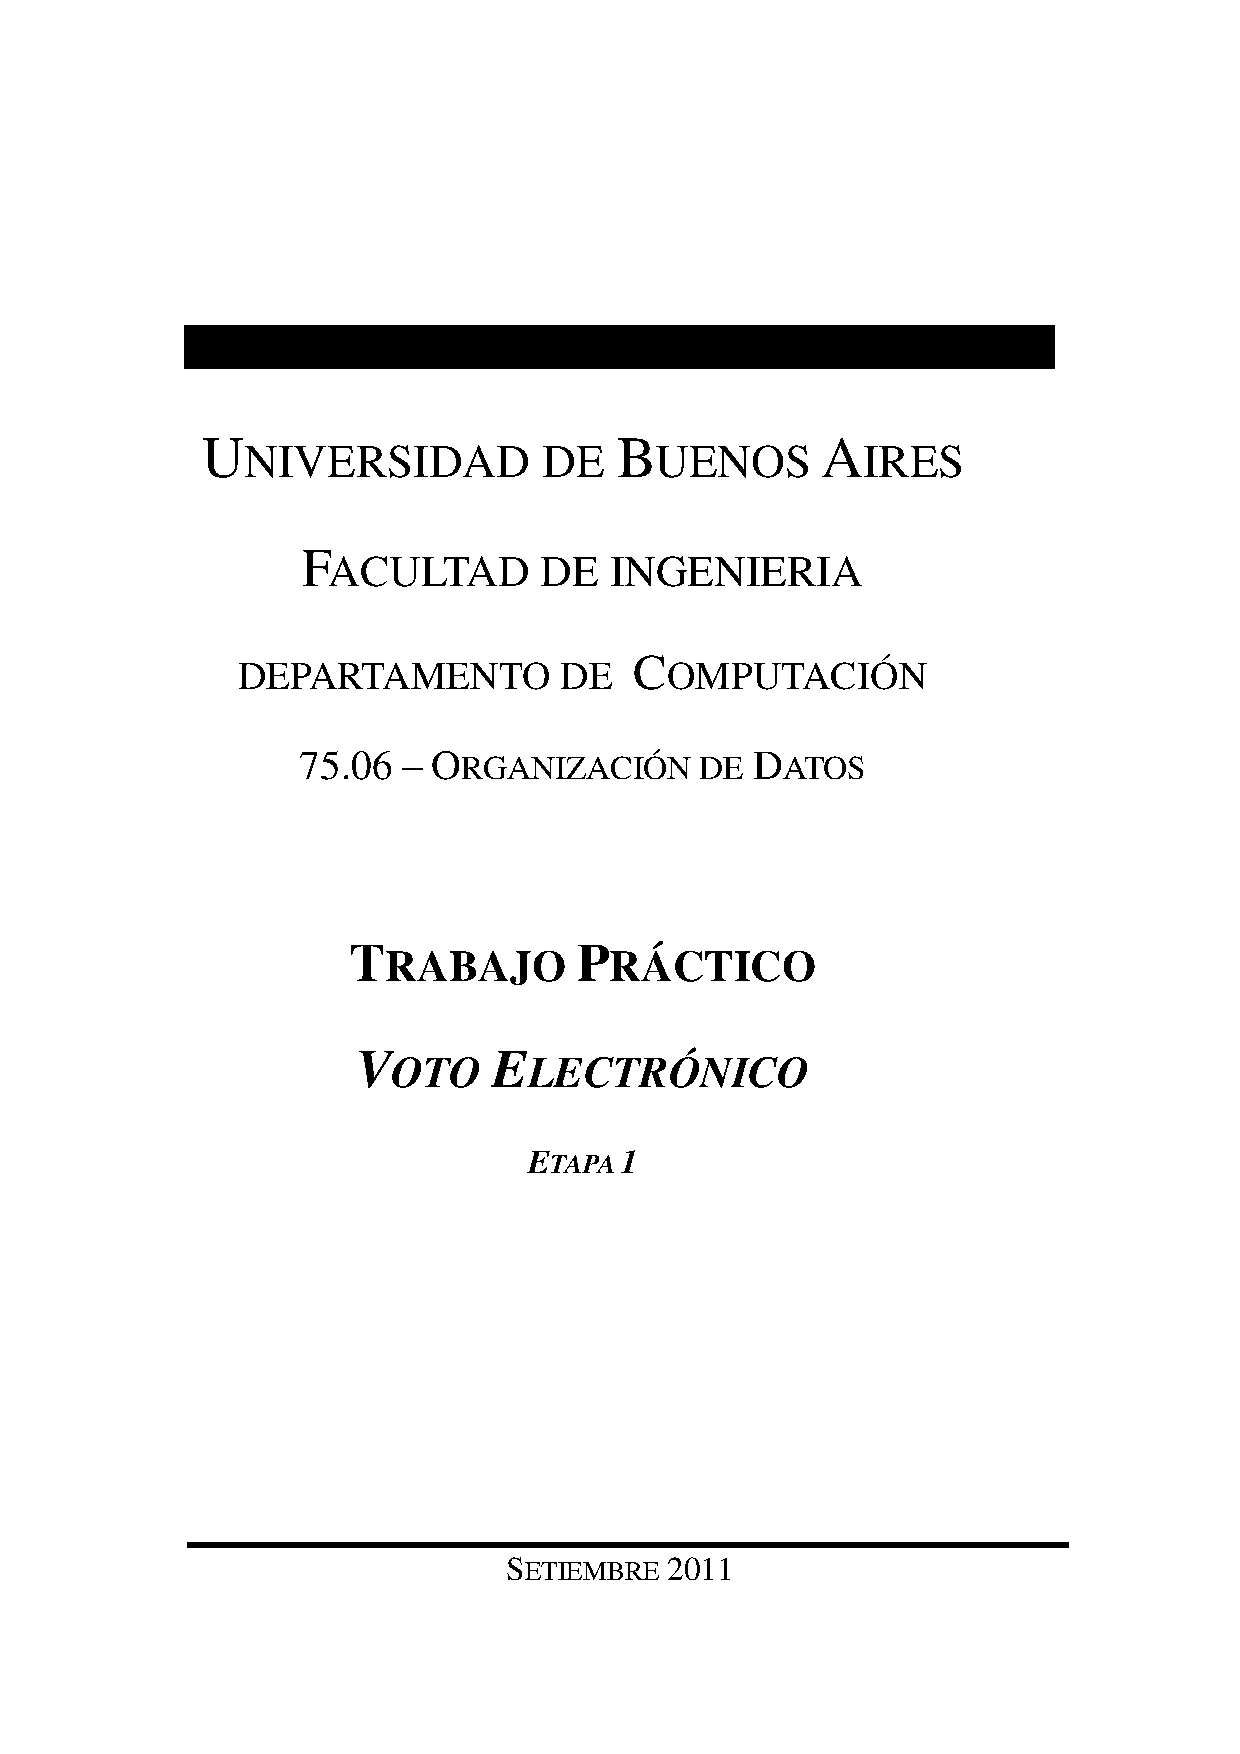
\includepdf[pages={1-10}]{./enunc.pdf}

\section{Apendice - Enunciado TP Etapa 2}
A continuación se agrega el enunciado de la Etapa 2, correspondiente a este Trabajo Práctico.
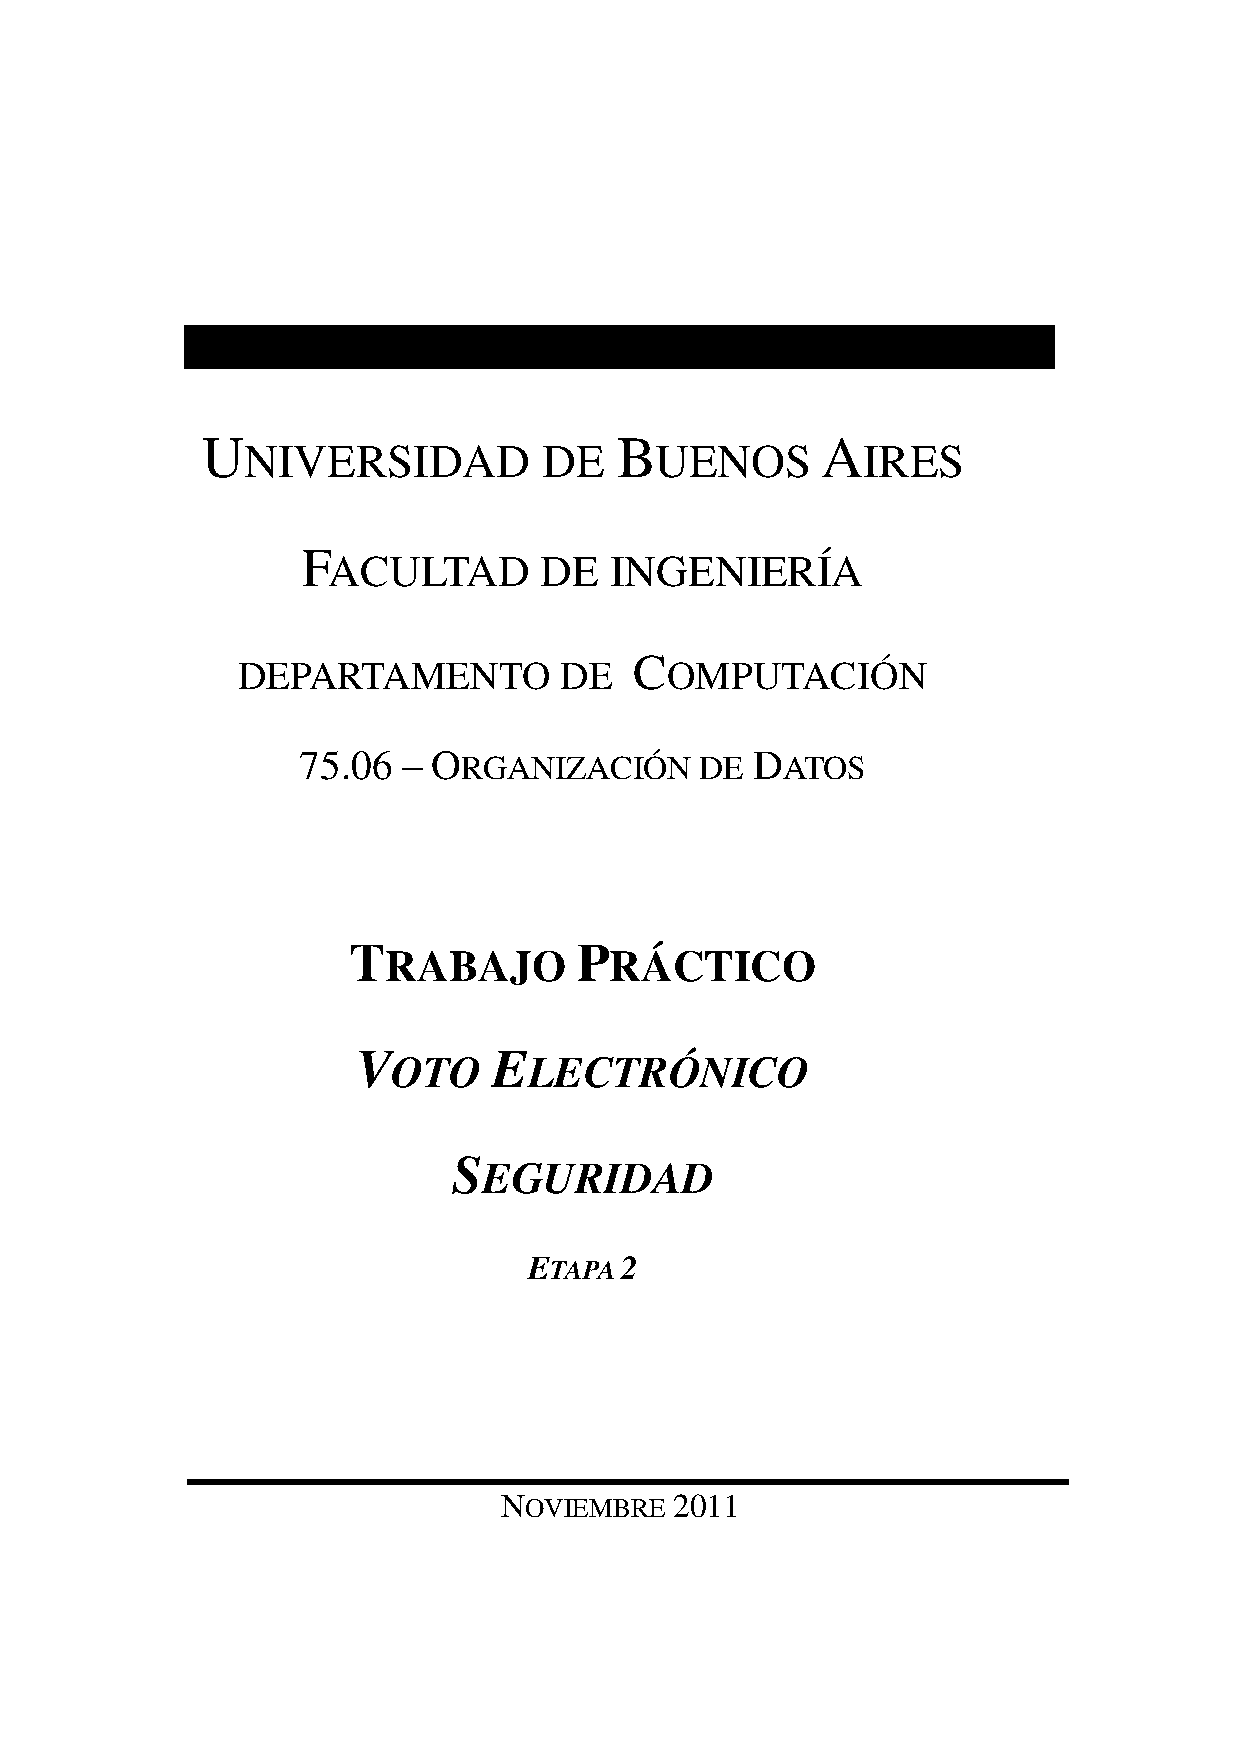
\includepdf[pages={1-6}]{./enunc2.pdf}


\end{document}

